\chapter{評価・実験}
本研究では,提案する視覚エフェクトと振動刺激の提示手法を用いた評価実験を行った.本章では実験内容およびその結果を示す.

評価.実験では,VR上に魔法の杖を表示しそこから数種類の形状の魔法を放ち、それに伴い振動モーターを振動させ,魔法の形状に対して振動パターンがユーザーの没入感にどのような影響を与えるのかを調査する.

\section{実験方法}
本章では作成したシステムを用いた評価実験を行った.
22歳の男性-名に対して実験を実施した.

被験者はヘッドマウントディスプレイを装着し右手にコントローラーを持つ.実験の様子を\figref{jikken}に示す.
提示する視覚エフェクトと振動パターンを実験者が選択する.この時被験者に選択したエフェクトを伝えておく.
視覚エフェクトに対して4パターンの振動刺激を提示した後アンケートを実施する.これを視覚エフェクトごとに繰り返す.
実験の被験者の視界を\figref{first}に示す.

\begin{figure}[h]
\centering
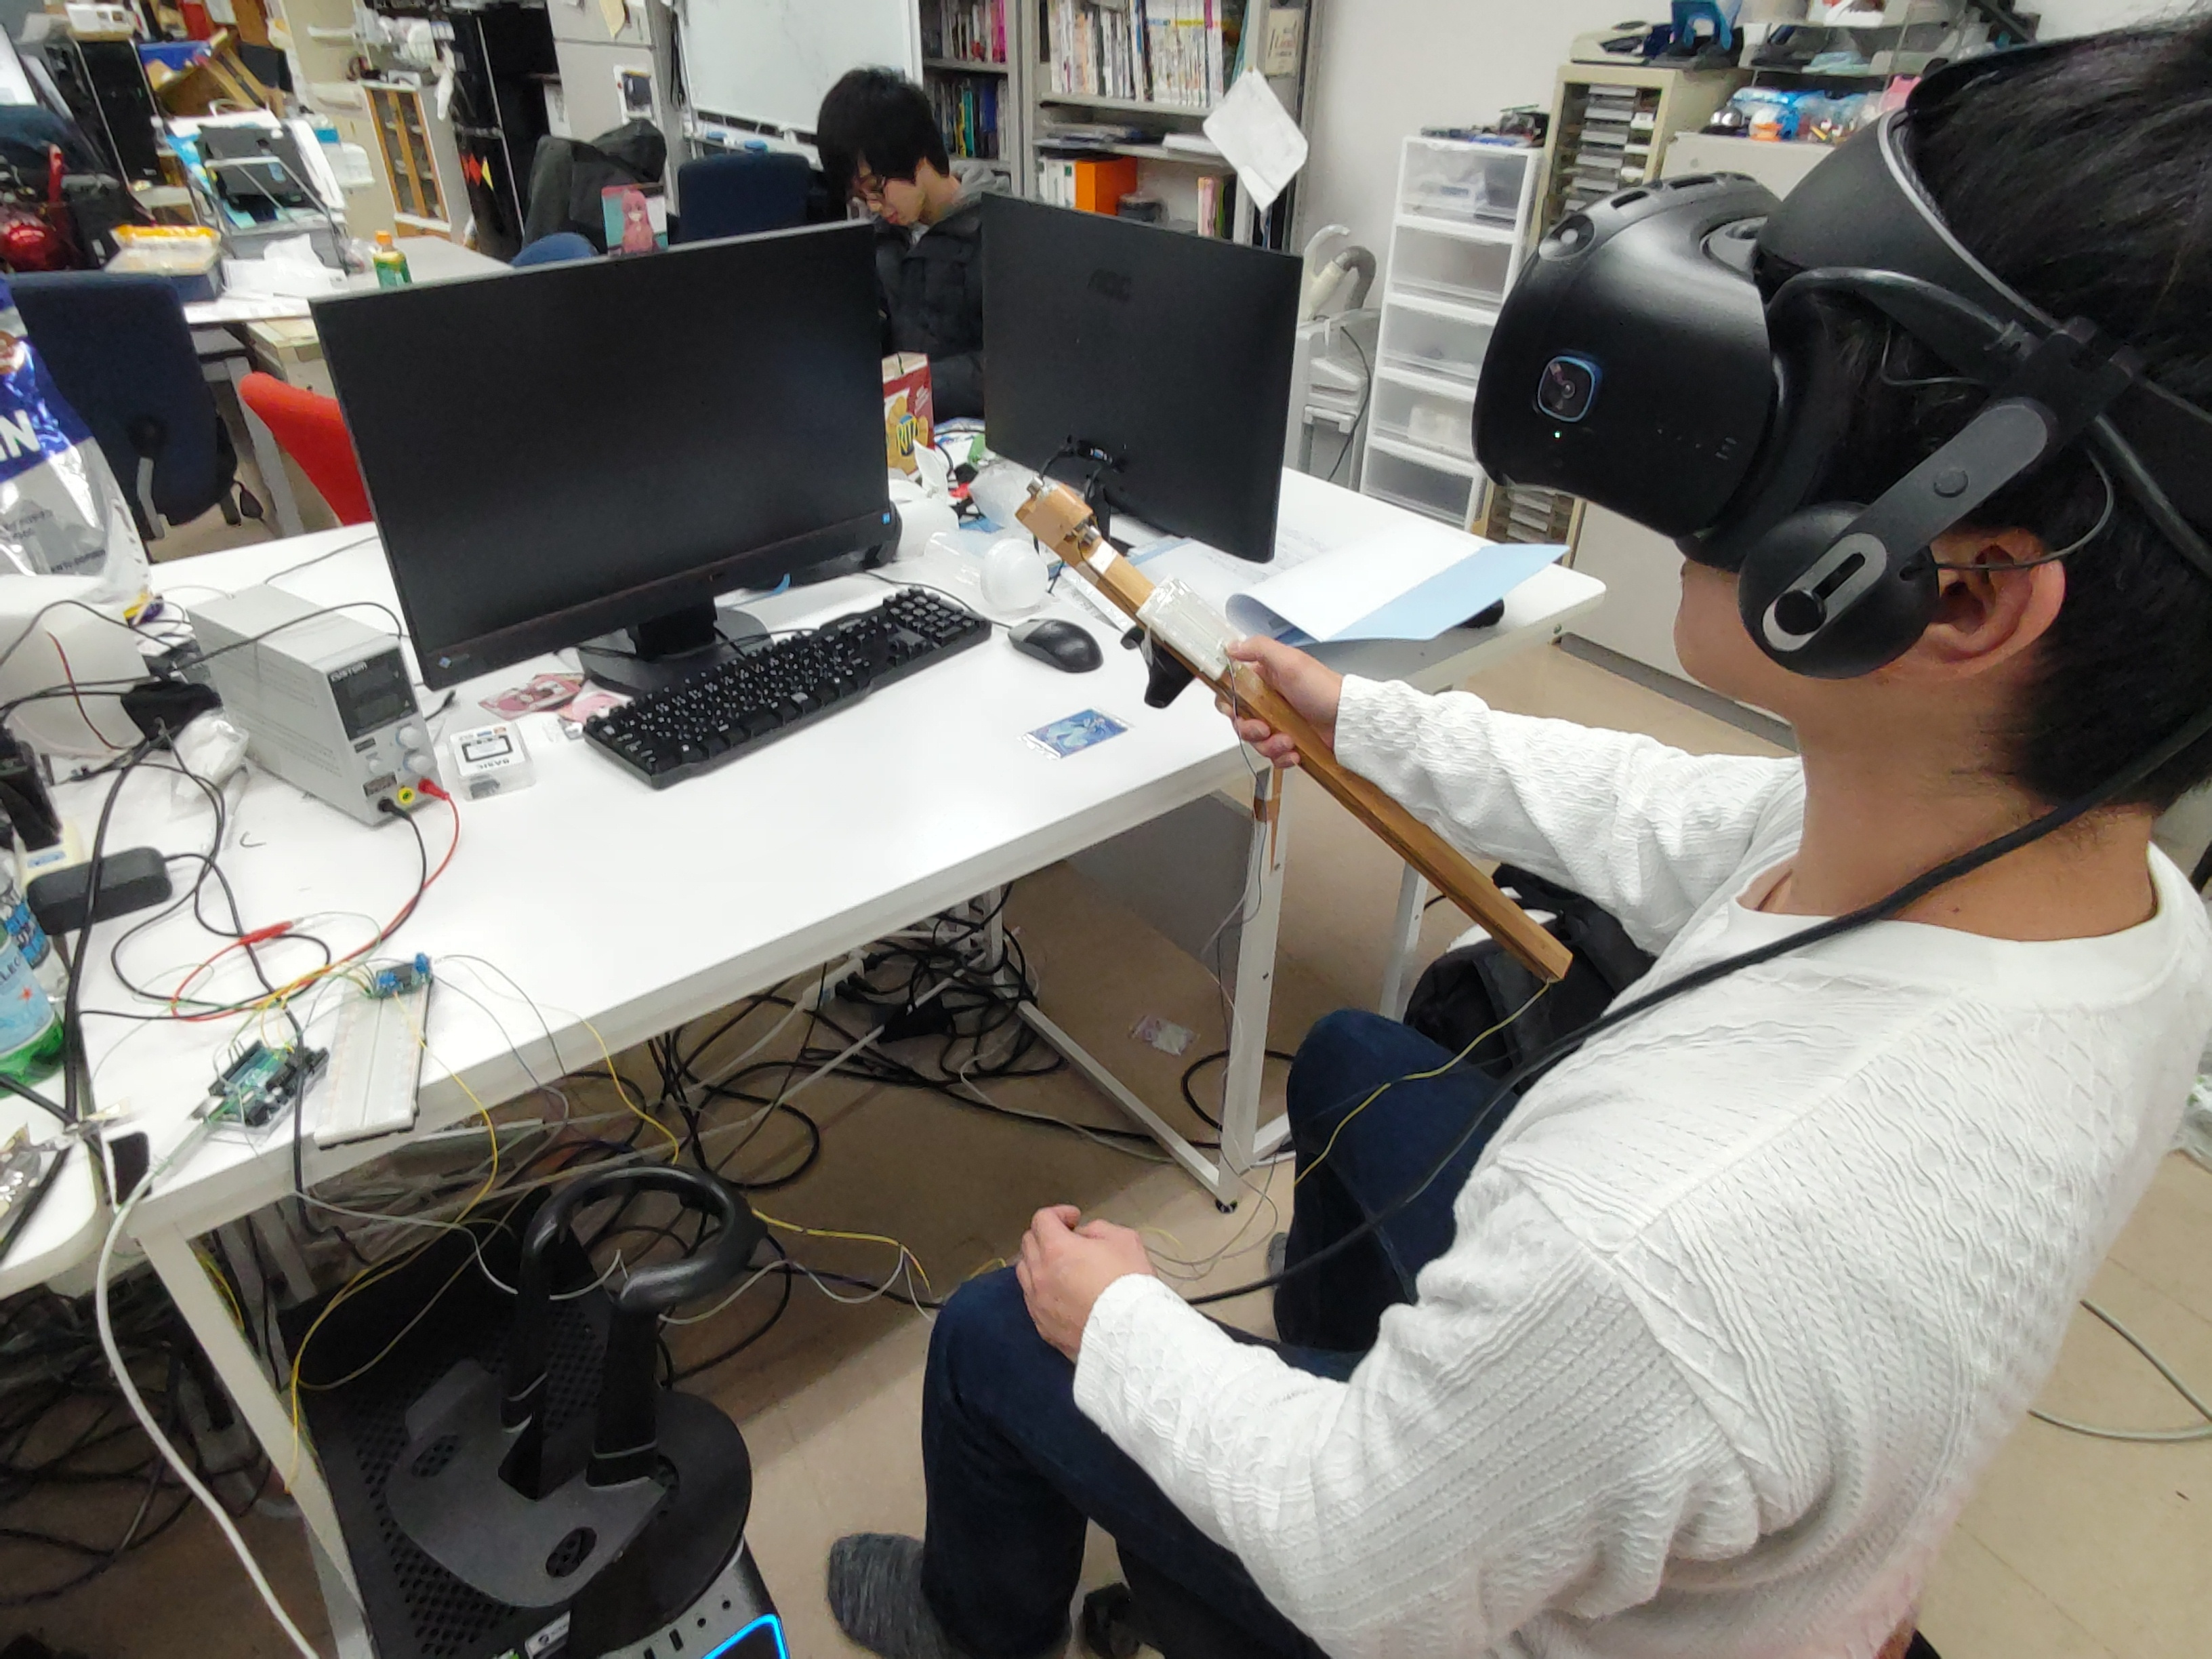
\includegraphics[clip,width=10cm]{./fig/jikken.JPG}
\caption{実験の様子}\label{jikken}
\end{figure}


\begin{figure}[h]
\centering
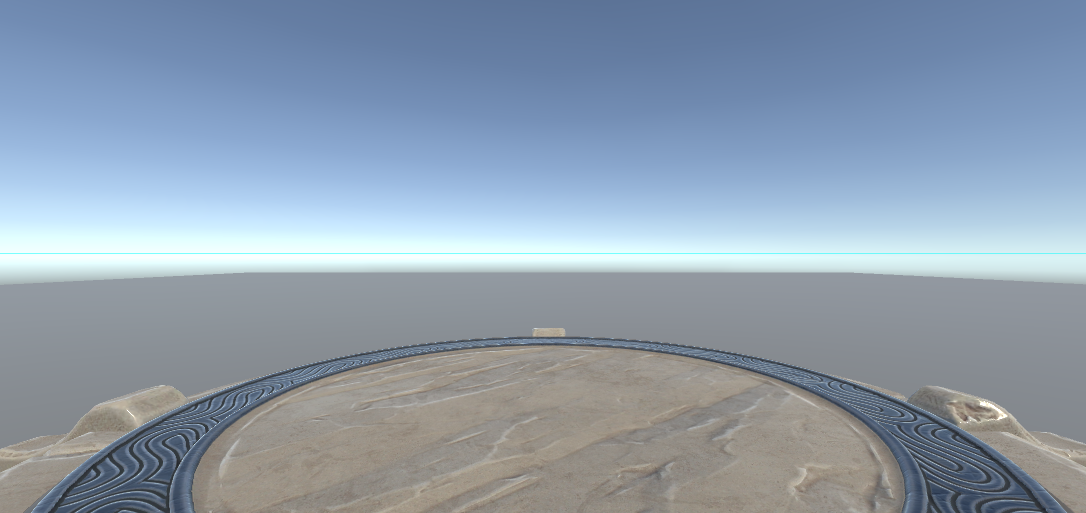
\includegraphics[clip,width=10cm]{./fig/unity_first.png}
\caption{実験者の視界}\label{first}
\end{figure}




\subsection{実験手順}
本実験の手順を以下に示す.この工程をringfire,explosion,fireの順番に3種類ずつ繰り返す.
\begin{enumerate}
    \item 実験説明
    \item 実験準備
    \item 実験前アンケート
    \item 実験本番
    \item 実験後アンケート
\end{enumerate}






\begin{table}[htbp]
    \centering
    \caption{実験終了後アンケート}
    \label{tab:後}
    {\renewcommand\arraystretch{1.2}}
    \begin{tabular}{l|l}
        \hline \hline
        問1 & あなたはこのシステムにどの程度関心を持ちましたか?\\
         問2 & どの程度システムに集中できましたか?\\
         問3 & どの程度システムに夢中になれましたか?\\
         問4 & システム使用中にどのくらい現実のことを意識し手いましたか?\\
         問5 & どの程度システム環境とインタラクションで来ていると感じましたか?\\
         問6 & 視覚エフェクトと振動刺激はどの程度一致していると感じましたか?\\
         問7 & 実際に自分が魔法を放っている感覚になりましたか?\\
         \hline
         
    \end{tabular}
\end{table}

\section{アンケート}
実験実施前と実施後にアンケートを行う.
実験前アンケートでは、まずこれから体験してもらう視覚エフェクトを見せ,用意した振動パターンのグラフから最もイメージに合うものを選択してもらった.

実験終了後にアンケートを行う.実験終了後アンケートを\ref{tab:後}に示す.実験終了後アンケートではシステムに没入できているか,振動刺激と視覚エフェクトが一致していたかなどこのデバイスの有用性を調査するために7項目の質問を5段階評価のアンケートを実施する.また,質問項目にない意見やシステムを使用した感想などは自由記述で回答させる.

\subsection{結果}
\subsection{考察}
